\chapter{Résultats}

\section{Générations de Bruits}

\subsection{Bruit de Perlin (figure~\ref{fig:perlin_ref})}
Le bruit de perlin est obtenu \textit{via} l'utilisation de LibNoise.

\begin{figure}[!ht]
    \begin{center}
	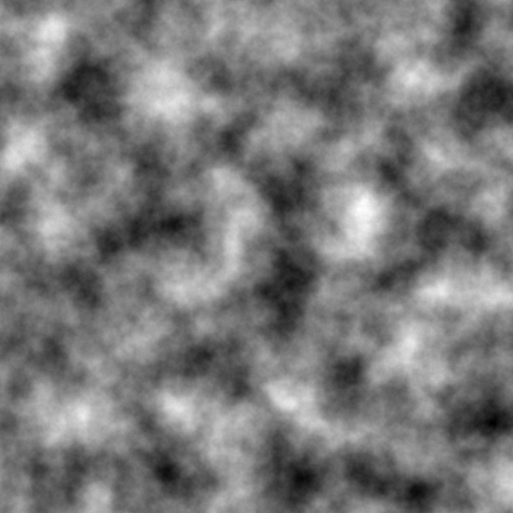
\includegraphics[width=5cm]{resources/perlin_ref.png}
        \caption{Bruit de Perlin}
        \label{fig:perlin_ref}	
    \end{center}
\end{figure}


\subsection{Bruit de Simplex (figure~\ref{fig:simplexnoise})}
Le bruit de simplex a été implémenté et permet d'obtenir des résultats satisfaisant. 
On remarque un effet de répétition et une faible variation locale de nuances (Contrairement au bruit de Perlin de LibNoise).
Cela est dû à un choix d'implémentation. Effectivement, nous sommes restés à une implémentation assez basique du bruit de Simplex.
Cela signifie que, contrairement à LibNoise, nous n'avons pas itéré N fois le bruit avec différentes amplitudes et fréquences.
Effectivement, le calcul des octaves est un ajout provenant de Fractional Brownian Motion.

\begin{figure}[!ht]
    \begin{center}
	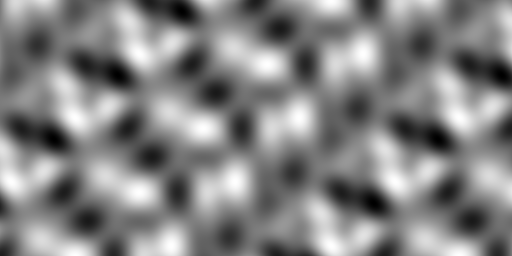
\includegraphics[width=10cm]{resources/simplexnoise.png}
        \caption{Bruit de Simplex}
        \label{fig:simplexnoise}
    \end{center}
\end{figure}

\section{Générations par méthodes Fractales}

\subsection{Midpoint Displacement (figure~\ref{fig:midpoint-displacementRef})}
Cette méthode fractale a été la première à être implémentée. Elle augmente la hauteur des points de 
façon progressive en partant du centre de la carte. Ainsi, on peut voir qu'il n'existera jamais de 
variation brutale des hauteurs avec cet algorithme. Ceci s'explique par sa méthode de calcul de la hauteur 
pondéré par les points adjacents.

\begin{figure}[!ht]
    \begin{center}
	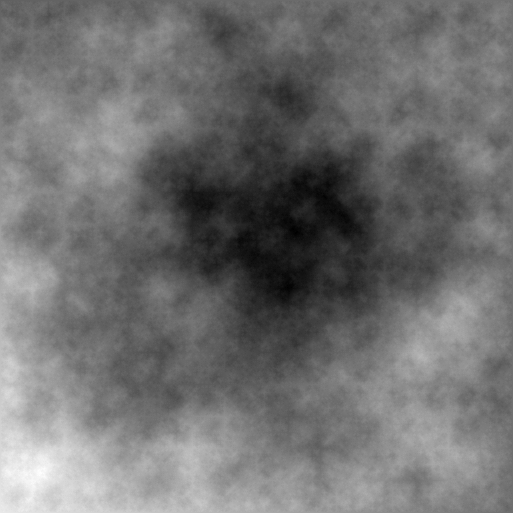
\includegraphics[width=5cm]{resources/midpoint_ref.png}
        \caption{Midpoint Displacement}
        \label{fig:midpoint-displacementRef}
    \end{center}
\end{figure}

\subsection{Diamond-Square (figure~\ref{fig:diamond_ref})}
Contrairement à Midpoint displacement, Diamond-Square propose plus de motifs mais cette méthode se 
base sur un calcul de moyennes avec une pondération par rapport aux hauteurs précédentes. 

\begin{figure}[!ht]
    \begin{center}
	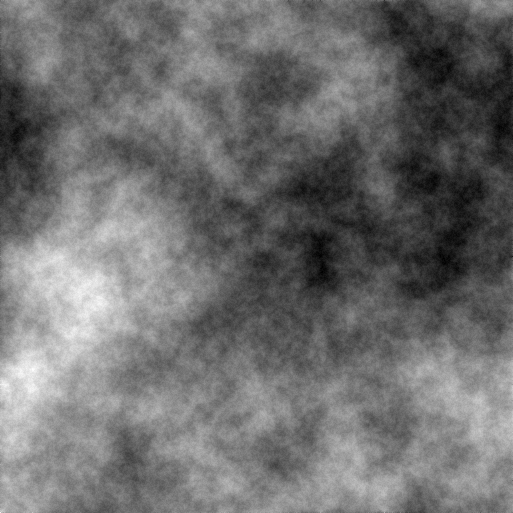
\includegraphics[width=5cm]{resources/diamond_ref.png}
         \caption{Diamond-Square}
         \label{fig:diamond_ref}
    \end{center}
\end{figure}

\section{Modèles d'érosions}
Deux modèles d'érosions sont présents dans la bibliothèque. 
L'une se nomme thermal erosion tandis que l'autre se nomme hydraulic erosion.
Les deux doivent méthodes modifient directement une carte d'élévation généré avec les méthodes cités précédemment.

\subsection{Erosion thermique (figure~\ref{fig:perlin_ref_thermal})}
L'érosion thermique simule la dégradation des reliefs avec la chute de matériaux 
vers le niveau le plus bas. Ainsi, une sensation de floue apparaît aux bordures des hauteurs.
Cet algorithme se base sur des comparaisons locales de la carte d'élévation pour altérer la hauteur de chaque sommet.
On peut voir les résultats obtenus sur le bruit de perlin ainsi que sur celui de simplex assez clairement.
On note également que la cohérence des cartes d'élévations sont les mêmes avec ou sans érosion thermique.
Cela signifie que la modification des hauteurs se calque bien sur un modèle de génération
d'où l'idée de ne pas faire un générateur d'érosion par type de carte d'élévation.

\begin{figure}[!ht]
  \begin{center}
	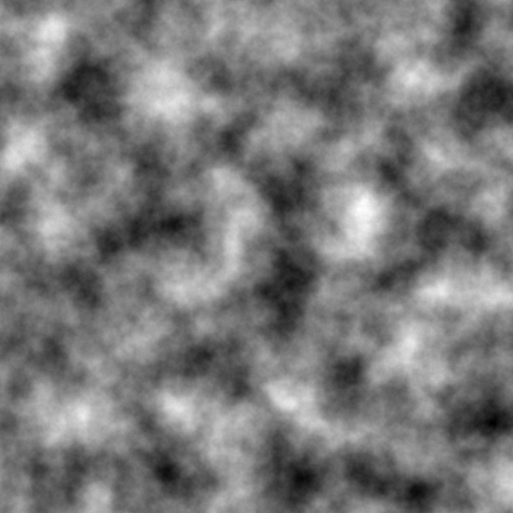
\includegraphics[width=5cm]{resources/perlin_ref.png}\hfill
	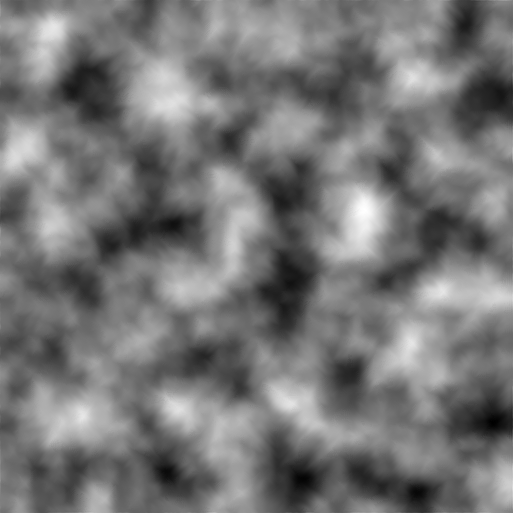
\includegraphics[width=5cm]{resources/perlin_thermalerosion.png}\hfill
        \caption{Bruit de Perlin sans érosion (gauche) et avec érosion thermique(droite)}
        \label{fig:perlin_ref_thermal}
        %%\label{fig:perlin_thermal}
        %% \caption{Bruit de Perlin avec érosion thermique}
   \end{center}
\end{figure}


\subsection{Erosion hydraulique (figure~\ref{fig:perlin_ref_hydraulic})}
L'érosion hydraulique simule plusieurs phénomènes à faible conséquence.
Effectivement, le but de ce modèle est d'apporter des 
modifications uniformes sur la carte donc la nécessité de ne pas trop accentuer des zones plus que d'autres.
Tout comme l'érosion thermique, on peut voir que l'algorithme se calque sur la carte d'élévation.

\begin{figure}[!ht]
  \begin{center}
	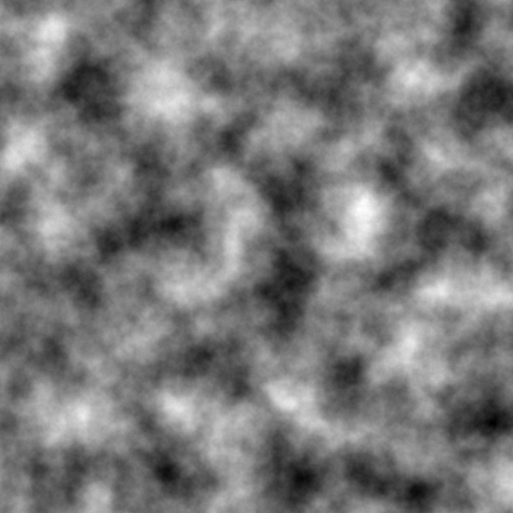
\includegraphics[width=5cm]{resources/perlin_ref.png}\hfill
	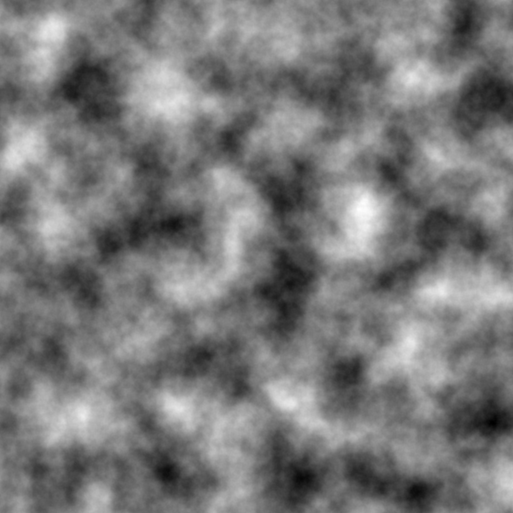
\includegraphics[width=5cm]{resources/perlin_hydraulicerosion.png}\hfill	
        \caption{Bruit de Perlin sans érosion (gauche) et avec érosion hydraulique(droite)}
        \label{fig:perlin_ref_hydraulic}
        %%\label{fig:perlin_thermal}
        %% \caption{Bruit de Perlin avec érosion thermique}
   \end{center}
\end{figure}

\section{Raffinement}
Il a été possible de raffiner localement une carte d'élévation en sélectionnant une zone de la carte.
Il ne s'agit, pour l'instant, que de modifier la valeur de pixels déjà présents. 
Nous n'avons pas encore implémenté de structures de données 
tels que les Quad-Tree pour augmenter le nombre de pixels sur une partie de la carte 
et donc augmenter le niveau de détail d'une zone donnée.

\section{Exports}
L'export des cartes d'élévations s'effectue sous différents formats : .pgm, .bmp et .ter.
L'export au format .pgm est relativement simple à mettre en place. 
Néanmoins, l'implémentation de celui-ci n'était pas spécifié dans le cahier des charges. 
Nous avons décidé d'implémenter cet export pour tester rapidement nous cartes d'élévation. 
Le format .bmp est très utilisé par les divers logiciels existants pour 
l'import et l'export d'une carte d'élévation. Le format .ter nous a permis de lire les cartes
d'élévation sous Terragen 3.
Les trois méthodes utilisent tous la même base de code c'est-à-dire qu'il y a une détection des valeurs 
maximale et minimale de la carte d'élévation dans l'objectif d'établir une échelle de gris.

\subsection{Format .pgm}
Nous n'avons pas eu besoin de bibliothèques particulière lors de l'implémentation de cet export.
Les résultats des tests concernant la cohérence des cartes d'élévation ainsi que les résultats
précédemment évoqués utilisent ce format d'export.

\subsection{Format .bmp}
Les images exportés au format .bmp sont les mêmes que celles au format.pgm. 
Ainsi, nous sommes sûr que l'export sur ce format est opérationnel.

\subsection{Format .ter}
L'export du fichier au format .ter nécessite d'écrire des en-têtes pour décrire les caractéristiques 
de la carte d'élévation. Enfin, les hauteurs de la carte d'élévation sont écrites en fin du fichier .ter.

\section{Compilation}
\subsection{Organisation}
Les fichiers du projet ont été séparés dans différents répertoires :
\begin{itemize}
 \item src/. Ce répertoire contient les fichiers sources du projet;
 \item test/. Ce répertoire contient les fichiers tests;
 \item samples/. Ce répertoire contient les exécutables produits lors de la compilation;
 \item doc/. Ce répertoire contient la documentation générable par doxygen.
\end{itemize}
Chaque répertoire possède un Makefile et un Makefile, situé à la racine du projet, permet de lire ces derniers.

\subsection{Utilisation}
La première etape est de faire \emph{./autogen.sh} et \emph{./configure} dans l'objectif de configurer et créer les fichiers
 makefile prêt. Ensuite, il est possible d'effectué différents type de \emph{make} :
 \begin{itemize}
  \item \emph{make} puis le nom de l'exécutable dans le dossier samples;
  \item \emph{make check} pour effectuer des tests;
  \item \emph{make doc} pour générer la documentation.
 \end{itemize}


%%\subsection{Format .obj}
